\documentclass[conference]{IEEEtran}
\IEEEoverridecommandlockouts
% The preceding line is only needed to identify funding in the first footnote. If that is unneeded, please comment it out.
\usepackage{cite}
\usepackage{amsmath,amssymb,amsfonts}
\usepackage{algorithmic}
\usepackage{graphicx}
\usepackage{textcomp}
\usepackage{xcolor}
\usepackage{booktabs}
\usepackage{dcolumn} % Booktabs column spacing
\usepackage{threeparttable} % Align column caption, table, and notes
\usepackage{adjustbox} % Shrink boxes
\usepackage{float}
\def\BibTeX{{\rm B\kern-.05em{\sc i\kern-.025em b}\kern-.08em
    T\kern-.1667em\lower.7ex\hbox{E}\kern-.125emX}}
\begin{document}

\title{Heart Disease Prediction}

\author{\IEEEauthorblockN{Xavier Santos}
    \IEEEauthorblockA{\textit{Departamento de Eletrónica, Telecomunicações e Informática} \\
        \textit{Universidade de Aveiro}\\
        Aveiro, Portugal \\
        xavier@ua.pt
    }
}

\maketitle

\begin{abstract}
    This project aims to find the most efficient model to predict the presence of a heart disease on a patient based on 14 preconditions and exam results from a single hospital and then test the trained models against data from hospitals in different hospitals and countries.
\end{abstract}

\begin{IEEEkeywords}
    machine learning, dataset, heart disease, prediction, logistic regression, naive Bayes, k nearest neighbors, decision tree, random forest
\end{IEEEkeywords}

\section{Introduction}
For this study, it was analyzed the data form the UCI Machine Learning Repository\cite{mlr} regarding patient data used to ascertain the presence of a heart disease. In order to predict said disease five models of prediction were used: Logistic Regression, Naive Bayes, K Nearest Neighbors, Decision Tree and Random Forest.

\section{Dataset}
The dataset used for training contains the data of 303 patients from a hospital in Cleveland\cite{va} described by 14 attributes each; 5 of which were numerical values while the other 9 represented categories. The "goal" field was given by a binary value representing the presence or absence of heart disease in the patient. There were other 3 other datasets from Hungary\cite{hun}, Switzerland\cite{swz1,swz2} and Long Beach\cite{va} in which the models obtained from the first set were tested after the training. Most of these datasets, however, had many missing values.\\
The features used are age, sex, chest pain type, resting blood pressure, cholesterol, fasting blood sugar, resting electrocardiogram, maximum heart rate, exercise induced angina, ST depression, ST slope, number of major vessels and Thallium stress test results. An example of a portion the data is show in Table \ref{data_head}.

\begin{table}[htbp]
    \caption{Data head}
    \begin{center}
        \resizebox{\columnwidth}{!}{%
            \begin{tabular}{lrrrrrrrrrrrrrr}
\toprule
{} &   Age &  Sex &  ChestPainType &  RestingBloodPressure &  Cholesterol &  FastingBloodSugar &  RestingECG &  MaxHeartRate &  ExerciseInducedAngina &  ST\_depression &  ST\_slope &  NumMajorVessels &  ThaliumStressTest &  Diagnosis \\
\midrule
0 &  63.0 &  1.0 &            1.0 &                 145.0 &        233.0 &                1.0 &         2.0 &         150.0 &                    0.0 &            2.3 &       3.0 &              0.0 &                6.0 &          0 \\
1 &  67.0 &  1.0 &            4.0 &                 160.0 &        286.0 &                0.0 &         2.0 &         108.0 &                    1.0 &            1.5 &       2.0 &              3.0 &                3.0 &          1 \\
2 &  67.0 &  1.0 &            4.0 &                 120.0 &        229.0 &                0.0 &         2.0 &         129.0 &                    1.0 &            2.6 &       2.0 &              2.0 &                7.0 &          1 \\
3 &  37.0 &  1.0 &            3.0 &                 130.0 &        250.0 &                0.0 &         0.0 &         187.0 &                    0.0 &            3.5 &       3.0 &              0.0 &                3.0 &          0 \\
4 &  41.0 &  0.0 &            2.0 &                 130.0 &        204.0 &                0.0 &         2.0 &         172.0 &                    0.0 &            1.4 &       1.0 &              0.0 &                3.0 &          0 \\
5 &  56.0 &  1.0 &            2.0 &                 120.0 &        236.0 &                0.0 &         0.0 &         178.0 &                    0.0 &            0.8 &       1.0 &              0.0 &                3.0 &          0 \\
6 &  62.0 &  0.0 &            4.0 &                 140.0 &        268.0 &                0.0 &         2.0 &         160.0 &                    0.0 &            3.6 &       3.0 &              2.0 &                3.0 &          1 \\
7 &  57.0 &  0.0 &            4.0 &                 120.0 &        354.0 &                0.0 &         0.0 &         163.0 &                    1.0 &            0.6 &       1.0 &              0.0 &                3.0 &          0 \\
8 &  63.0 &  1.0 &            4.0 &                 130.0 &        254.0 &                0.0 &         2.0 &         147.0 &                    0.0 &            1.4 &       2.0 &              1.0 &                7.0 &          1 \\
9 &  53.0 &  1.0 &            4.0 &                 140.0 &        203.0 &                1.0 &         2.0 &         155.0 &                    1.0 &            3.1 &       3.0 &              0.0 &                7.0 &          1 \\
\bottomrule
\end{tabular}

        }%
        \label{data_head}
    \end{center}
\end{table}

\section{Data analysis}

There is some information that can be gathered from a preliminary analysis of the data. Like the distribution of diseased patients by age, sex or any other attribute.

\begin{figure}[htbp]
    \centerline{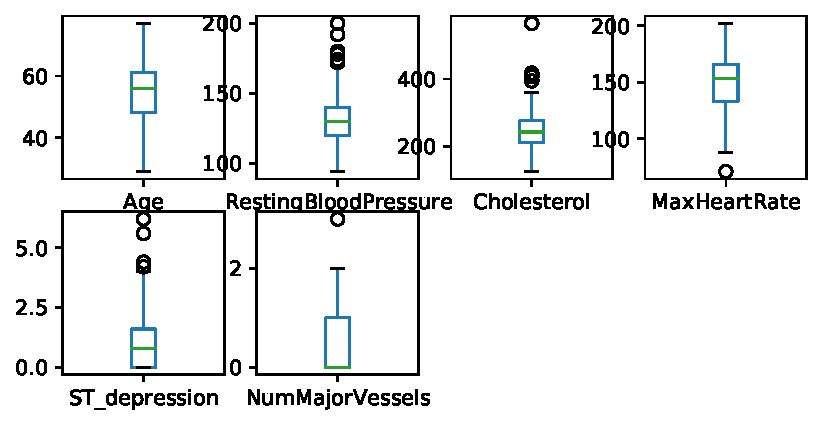
\includegraphics[width=0.7\linewidth]{images/age_distribution.pdf}}
    \caption{Distribution of heart disease by patient's age}
    \label{age_dist}
\end{figure}

For example, in Figure \ref{age_dist} we can see that, in this sample, most of the cases of heart disease come from patients between 55 and 60 years old.

\begin{figure}[H]
    \centerline{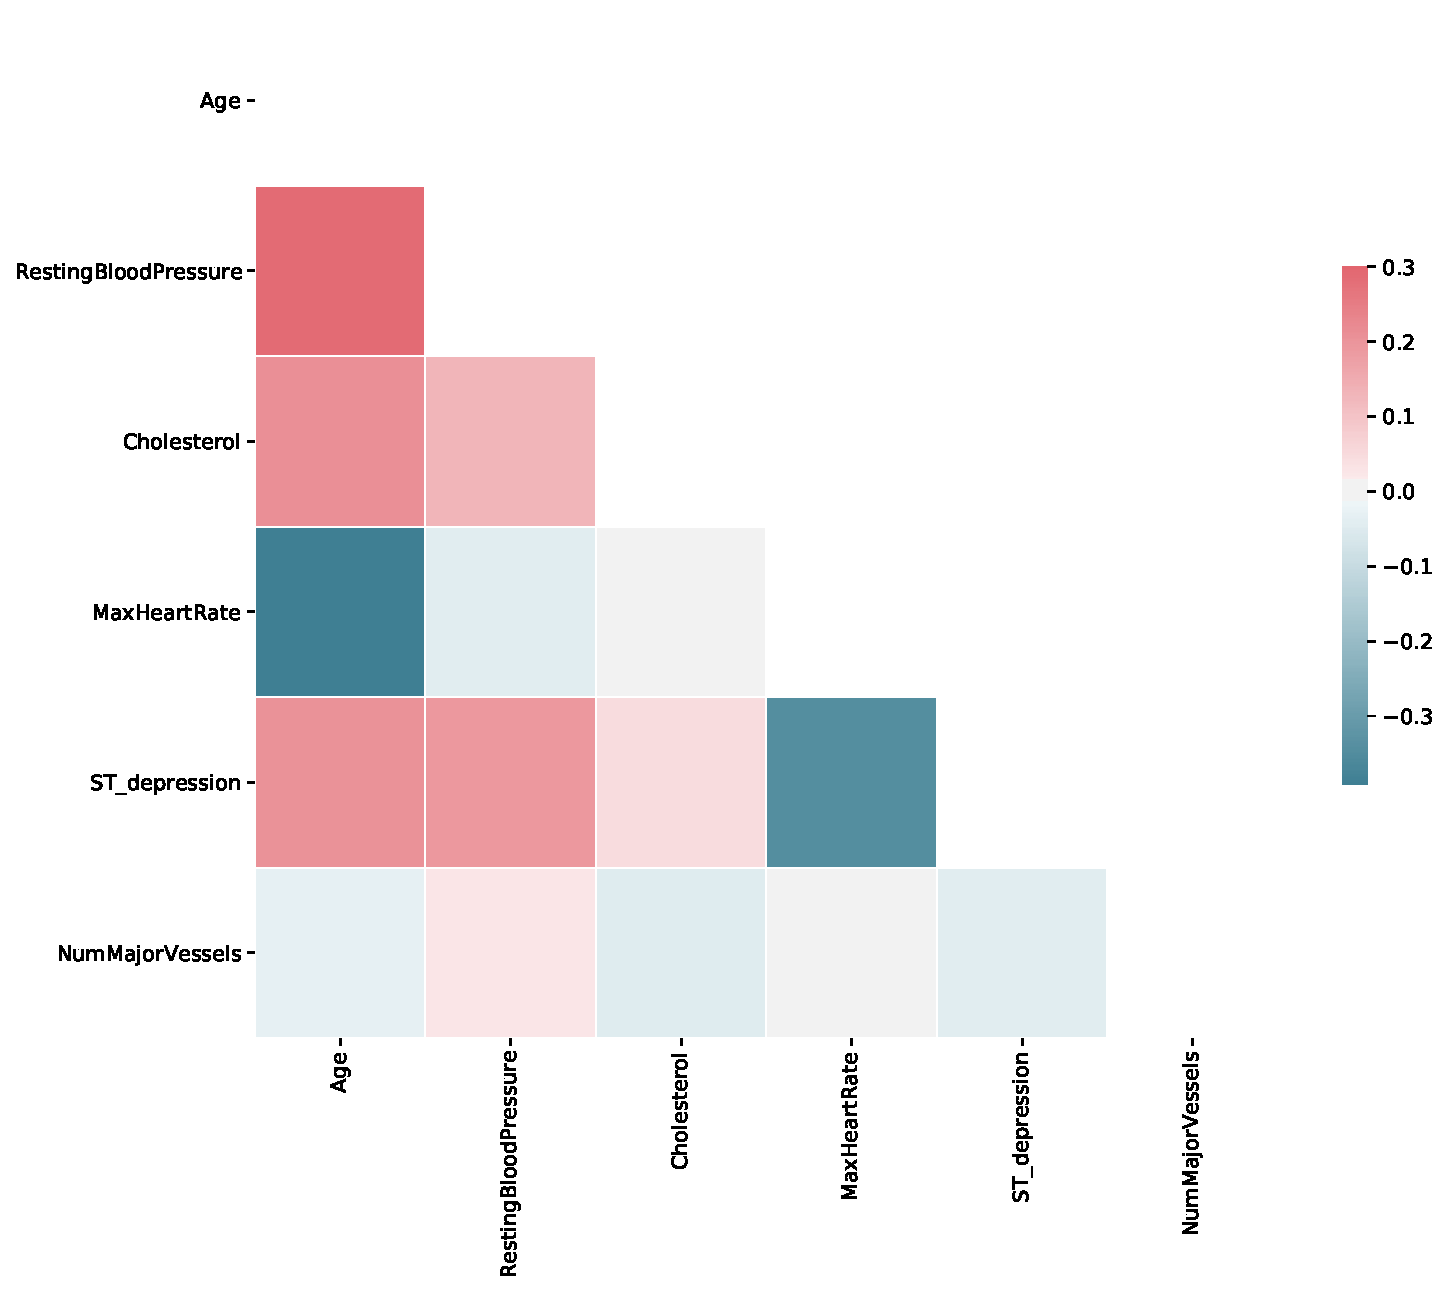
\includegraphics[width=0.7\linewidth]{images/correlation_heatmap.pdf}}
    \caption{Heat map of the correlation between the features and the diagnosis}
    \label{corr_heatmap}
\end{figure}

But what interests us the most is the relation between this attributes (features) and a case of heart disease(goal).
\\It was verified that some features have more impact on the patient's diagnosis than others. For instance, if a patient has or not exercise induced angina is a much stronger indicator of a heart disease than his number of major vessels or fasting blood sugar value as it can be seen in Table \ref{data_corr} and Figures \ref{corr_heatmap} and \ref{corr_scatter}.

\begin{table}[htbp]
    \caption{Data correlation}
    \begin{center}
        \begin{tabular}{lr}
\toprule
{} &  Diagnosis \\
\midrule
Diagnosis             &   1.000000 \\
ThalliumStressTest    &   0.526640 \\
NumMajorVessels       &   0.463189 \\
ST\_depression         &   0.424052 \\
MaxHeartRate          &   0.423817 \\
ExerciseInducedAngina &   0.421355 \\
ChestPainType         &   0.408945 \\
ST\_slope              &   0.333049 \\
Sex                   &   0.278467 \\
Age                   &   0.227075 \\
RestingECG            &   0.166343 \\
RestingBloodPressure  &   0.153490 \\
Cholesterol           &   0.080285 \\
FastingBloodSugar     &   0.003167 \\
\bottomrule
\end{tabular}

        \label{data_corr}
    \end{center}
\end{table}

\begin{figure}[H]
    \centerline{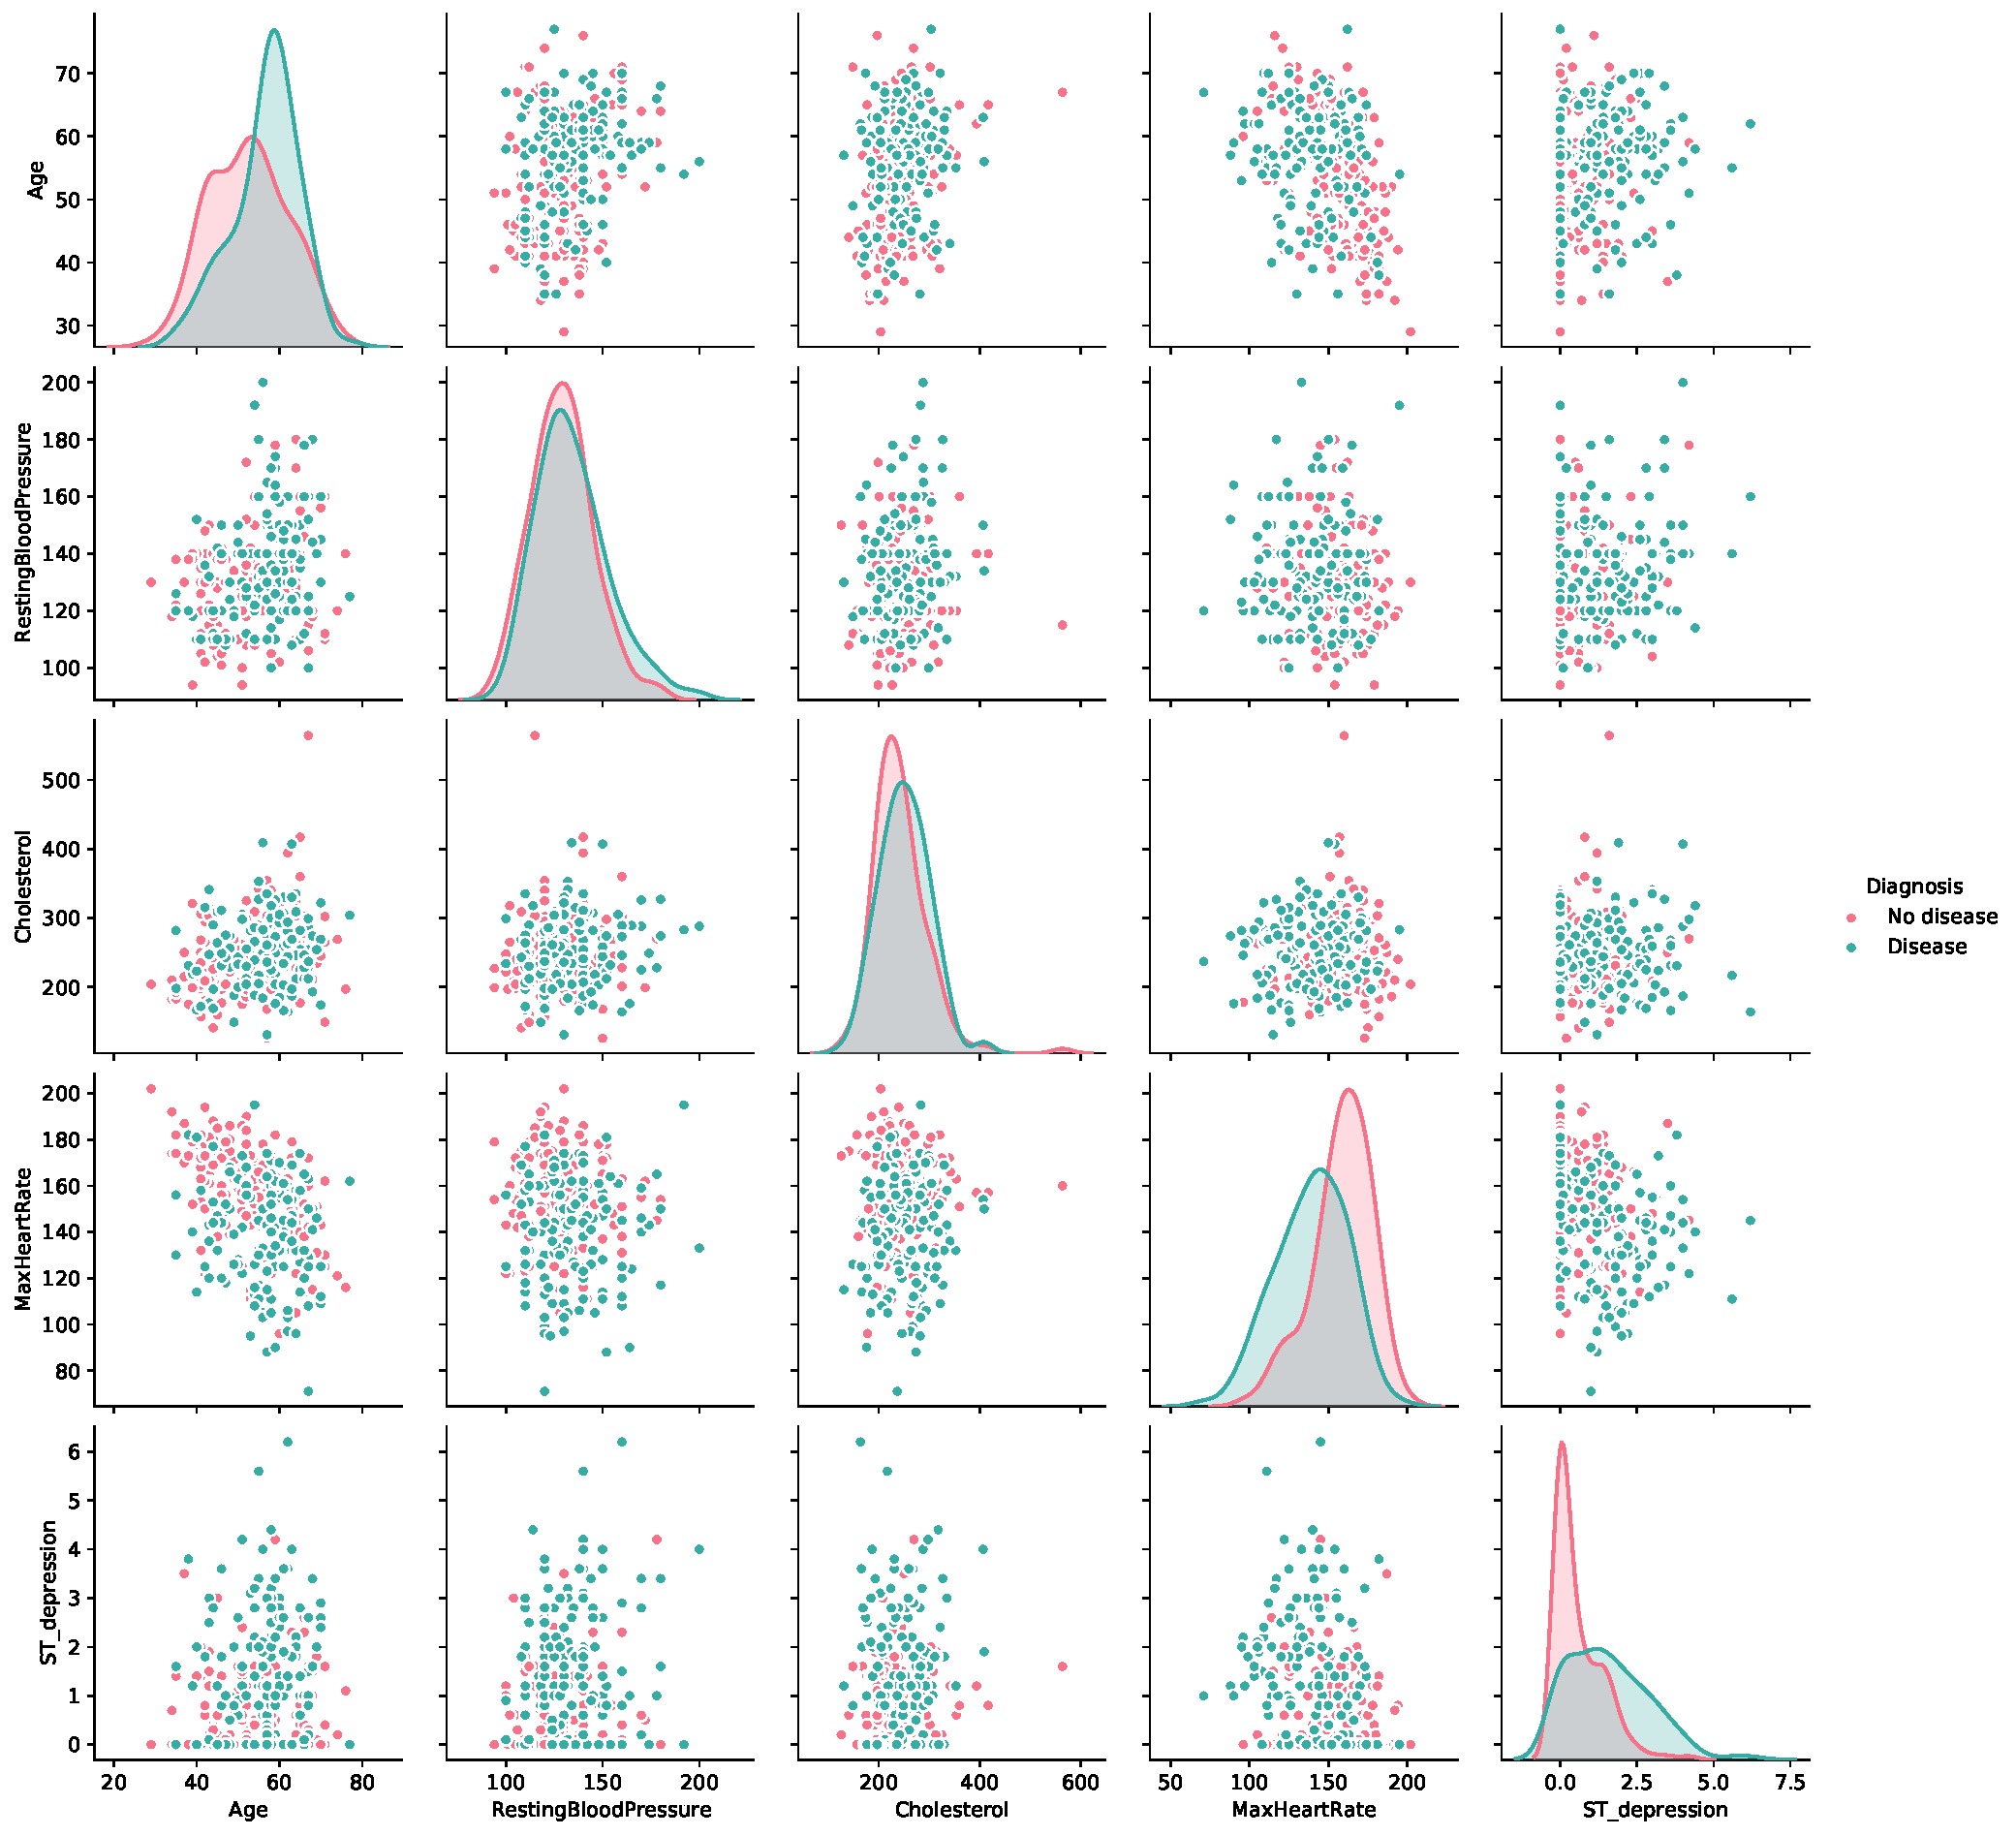
\includegraphics[width=\linewidth]{images/correlation_scatter.pdf}}
    \caption{Scatter plots of the correlation between the features and the diagnosis}
    \label{corr_scatter}
\end{figure}

\section{Data Preprocessing}
The data is provided by the UCI Machine Learning Repository\cite{mlr} in the format of a CSV file with the classifiers encoded into integers. The target is transformed from 5 different values for different heart disease to a binary value of diseased or not diseased.\\
Before training the models the data had to be prepared by filling the missing values on some of the features. This was achieved by giving the mean value for that feature if it was a numeric value or the most common value if it was categorical.\\
The data was then shuffled and split in two sets: one for training and another one for testing and cross-validation with the distribution of 80\% and 20\% respectively.

\section{Model training and tuning}

\subsection{Logistic Regression}
The logistic regression model uses a "liblinear" solver as it provides better results with smaller datasets and the goal we are taking in consideration is binary (disease / no disease).

\begin{figure}[H]
    \centerline{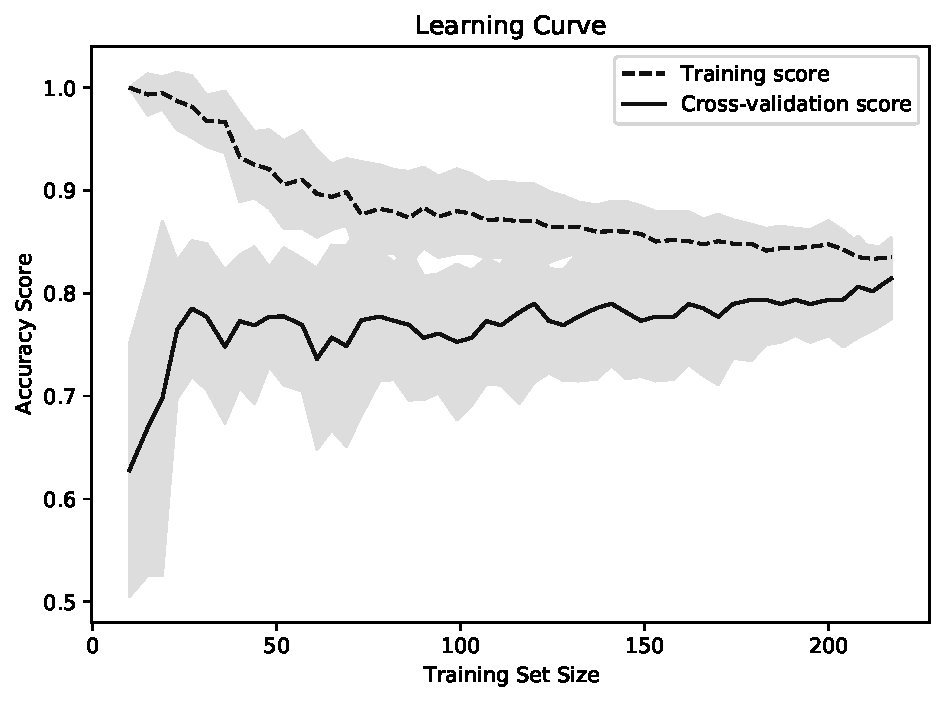
\includegraphics[width=0.9\linewidth]{images/LogisticRegression_lc.pdf}}
    \caption{Logistic Regression Learning Curve}
    \label{lr_lc}
\end{figure}

\noindent
Train accuracy: 86.36%
\\Test accuracy: 80.33%
\\Number of mislabeled points out of a total 61 points : 12
\\The accuracy score achieved is: 80.33 %
\begin{table}[H]
\caption{Classification report on full data set:}
\begin{center}
\begin{tabular}{lrrrr}
\toprule
{} &  precision &  recall &  f1-score &  support \\
\midrule
0            &       0.78 &    0.91 &      0.84 &    35.00 \\
1            &       0.85 &    0.65 &      0.74 &    26.00 \\
accuracy     &       0.80 &    0.80 &      0.80 &     0.80 \\
macro avg    &       0.82 &    0.78 &      0.79 &    61.00 \\
weighted avg &       0.81 &    0.80 &      0.80 &    61.00 \\
\bottomrule
\end{tabular}

\label{log_reg_class}
\end{center}
\end{table}
\noindent
False Negative Rate: 34.62
\\False Positive Rate: 8.57


\begin{figure}[H]
    \centerline{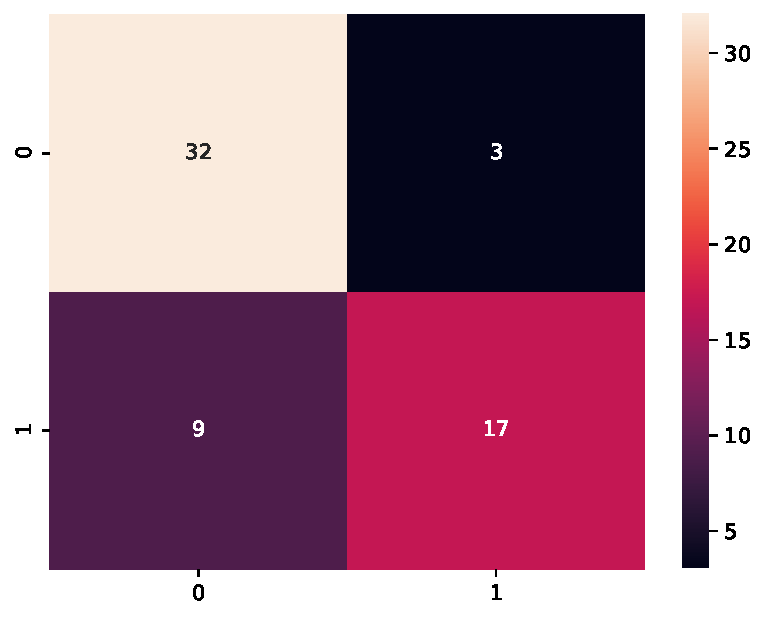
\includegraphics[width=0.8\linewidth]{images/log_reg_cm.pdf}}
    \caption{Logistic Regression Confusion Matrix}
    \label{lr_cm}
\end{figure}

\subsection{Naive Bayes}
Both the Gaussian and Bernoulli variants of the model were tested, but Bernoulli gave the best results. The Bernoulli method deals in binary inputs and transforms the rest of the data to binary-valued feature vectors. It is based on the formula:
\\[\baselineskip]
\centerline{$P(x_i \mid y) = P(i \mid y) x_i + (1 - P(i \mid y)) (1 - x_i)$}
\\[\baselineskip]
which means it penalizes the non-occurrence of a feature.

\begin{figure}[H]
    \centerline{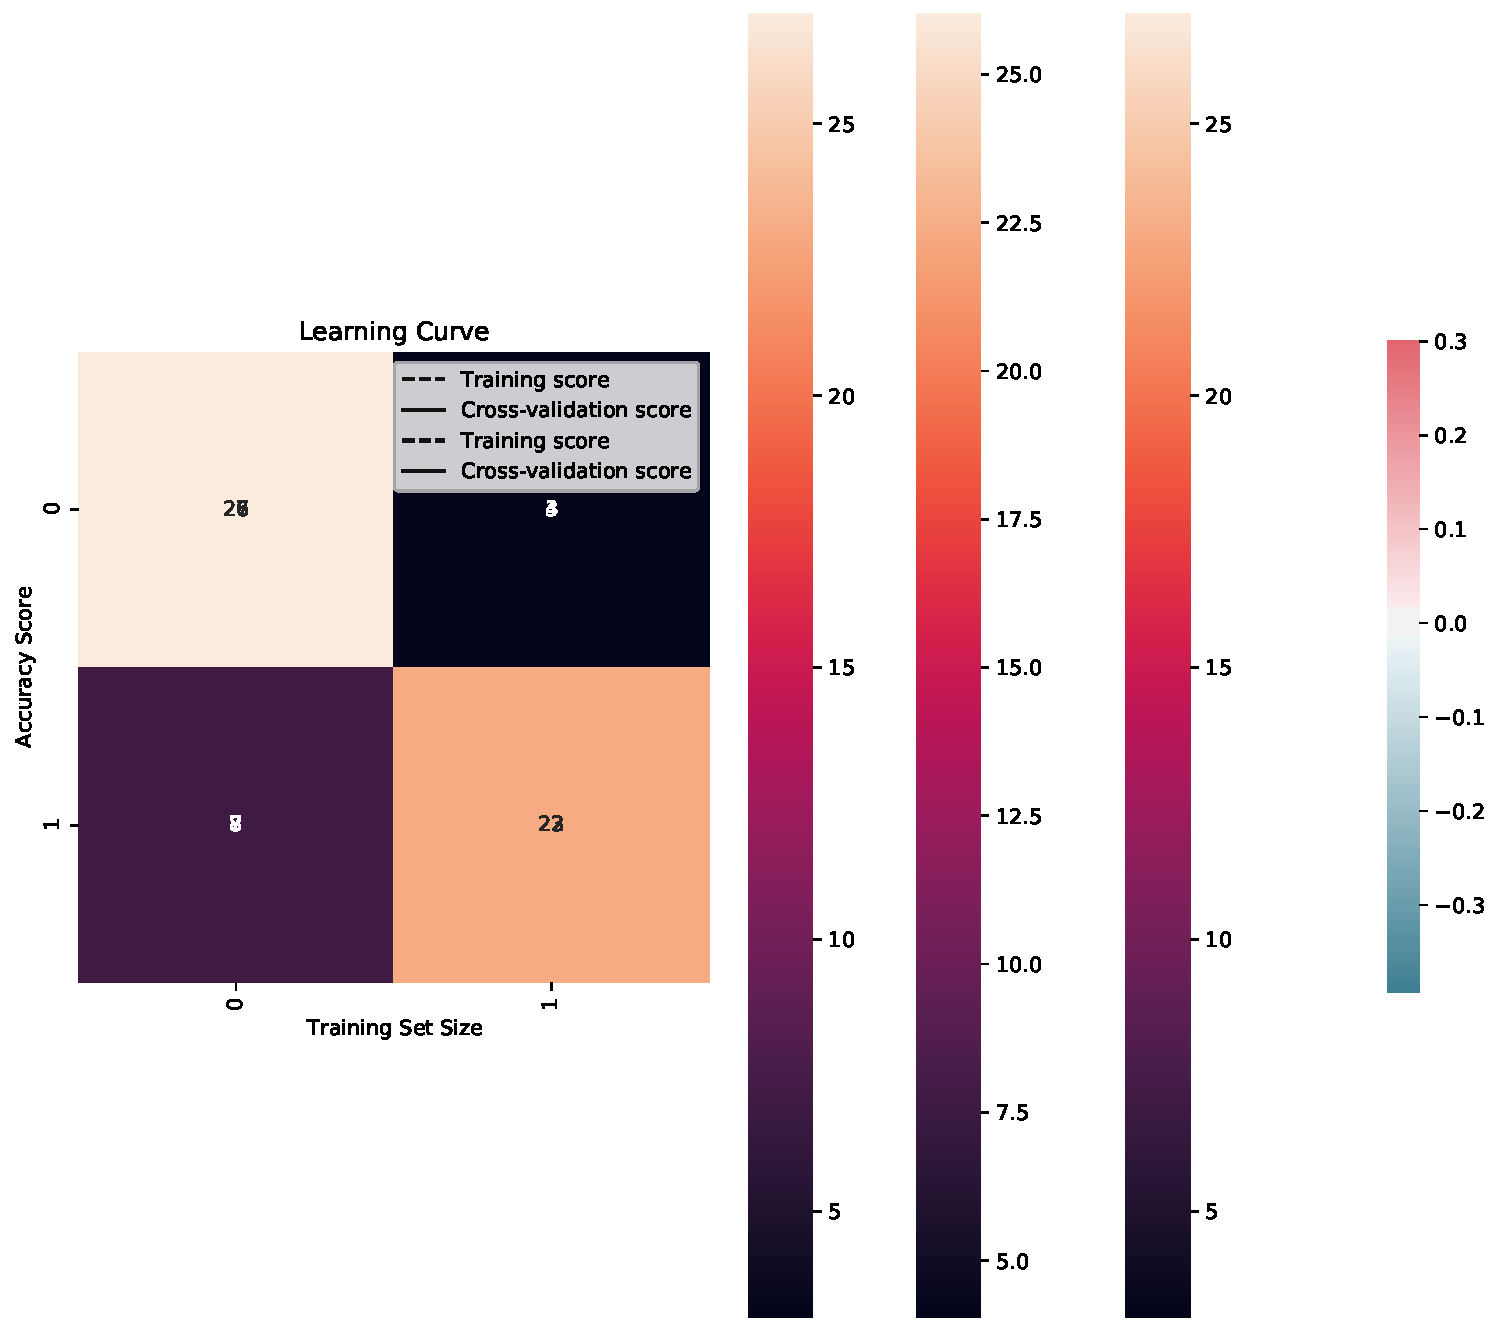
\includegraphics[width=0.9\linewidth]{images/BernoulliNB_lc.pdf}}
    \caption{Naive Bayes Learning Curve}
    \label{nb_lc}
\end{figure}

\noindent
Train accuracy: 80.17%
\\Test accuracy: 75.41%
\\Number of mislabeled points out of a total 61 points : 15
\\The accuracy score achieved is: 75.41 %
\begin{table}[H]
\caption{Classification report on full data set:}
\begin{center}
\begin{tabular}{lrrrr}
\toprule
{} &  precision &  recall &  f1-score &  support \\
\midrule
0            &       0.78 &    0.80 &      0.79 &    35.00 \\
1            &       0.72 &    0.69 &      0.71 &    26.00 \\
accuracy     &       0.75 &    0.75 &      0.75 &     0.75 \\
macro avg    &       0.75 &    0.75 &      0.75 &    61.00 \\
weighted avg &       0.75 &    0.75 &      0.75 &    61.00 \\
\bottomrule
\end{tabular}

\label{naive_bayes_class}
\end{center}
\end{table}
\noindent
False Negative Rate: 30.77
\\False Positive Rate: 20.00


\begin{figure}[H]
    \centerline{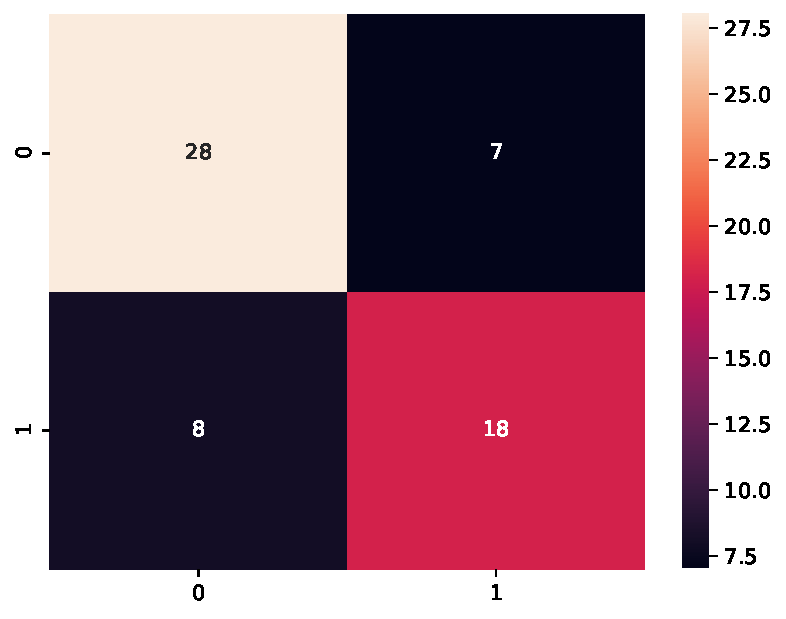
\includegraphics[width=0.8\linewidth]{images/naive_bayes_cm.pdf}}
    \caption{Naive Bayes Confusion Matrix}
    \label{nb_cm}
\end{figure}

\subsection{K Nearest Neighbors}
The optimal choice of the value of \textit{K} is highly data-dependent: in general a larger suppresses the effects of noise, but makes the classification boundaries less distinct. This model implements learning based on the \textit{K} nearest neighbors of each query point, where \textit{K} was selected from testing multiple candidates of which \textit{K}=3 gave the best results for the test set.

\begin{figure}[H]
    \centerline{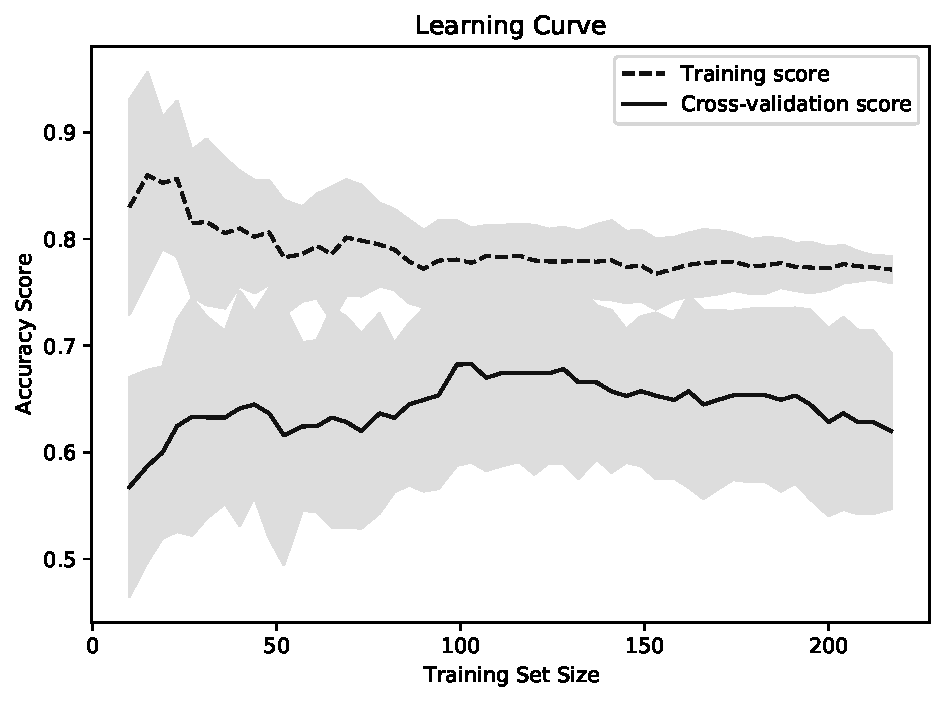
\includegraphics[width=0.9\linewidth]{images/KNeighborsClassifier_lc.pdf}}
    \caption{K Nearest Neighbors Learning Curve}
    \label{knn_lc}
\end{figure}

\noindent
N neighbors = 2\\
Train accuracy: 76.45%
\\Test accuracy: 68.85%
\\Number of mislabeled points out of a total 61 points : 19
\\The accuracy score achieved is: 68.85 %
\begin{table}[H]
\caption{Classification report on full data set:}
\begin{center}
\begin{tabular}{lrrrr}
\toprule
{} &  precision &  recall &  f1-score &  support \\
\midrule
0            &       0.68 &    0.86 &      0.76 &    35.00 \\
1            &       0.71 &    0.46 &      0.56 &    26.00 \\
accuracy     &       0.69 &    0.69 &      0.69 &     0.69 \\
macro avg    &       0.69 &    0.66 &      0.66 &    61.00 \\
weighted avg &       0.69 &    0.69 &      0.67 &    61.00 \\
\bottomrule
\end{tabular}

\label{k_nearest_neighbors_class}
\end{center}
\end{table}
\noindent
False Negative Rate: 53.85
\\False Positive Rate: 14.29


\begin{figure}[H]
    \centerline{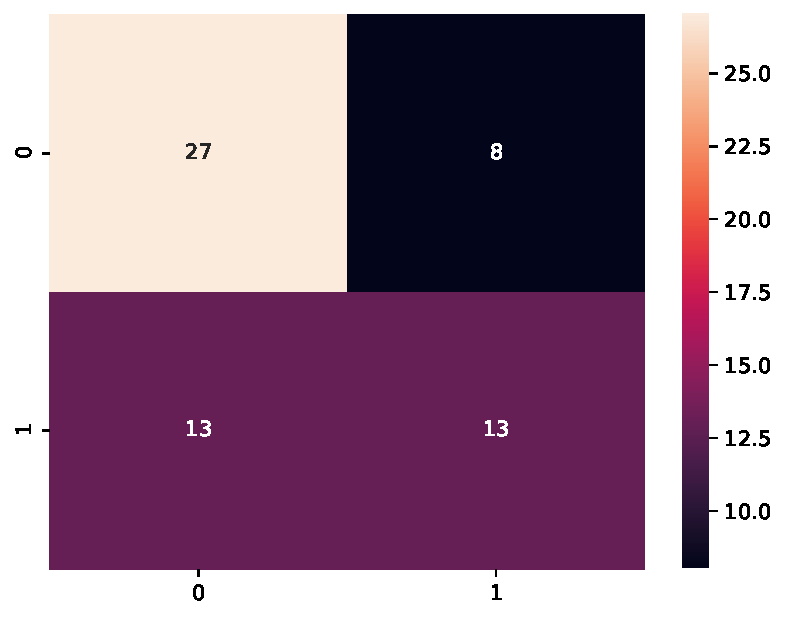
\includegraphics[width=0.8\linewidth]{images/k_nearest_neighbors_cm.pdf}}
    \caption{K Nearest Neighbors Confusion Matrix}
    \label{knn_cm}
\end{figure}

\subsection{Decision Tree}
This model predicts the value of a target variable using simple if-then-else rules inferred from the data features. This decisions can be made on different levels (depth) until reaching the target goal.
\\For the selection of the maximum depth of the decision tree classifier were tested the values from 1 to 10 and the chosen the one which gave best results for the test subset.

\begin{figure}[H]
    \centerline{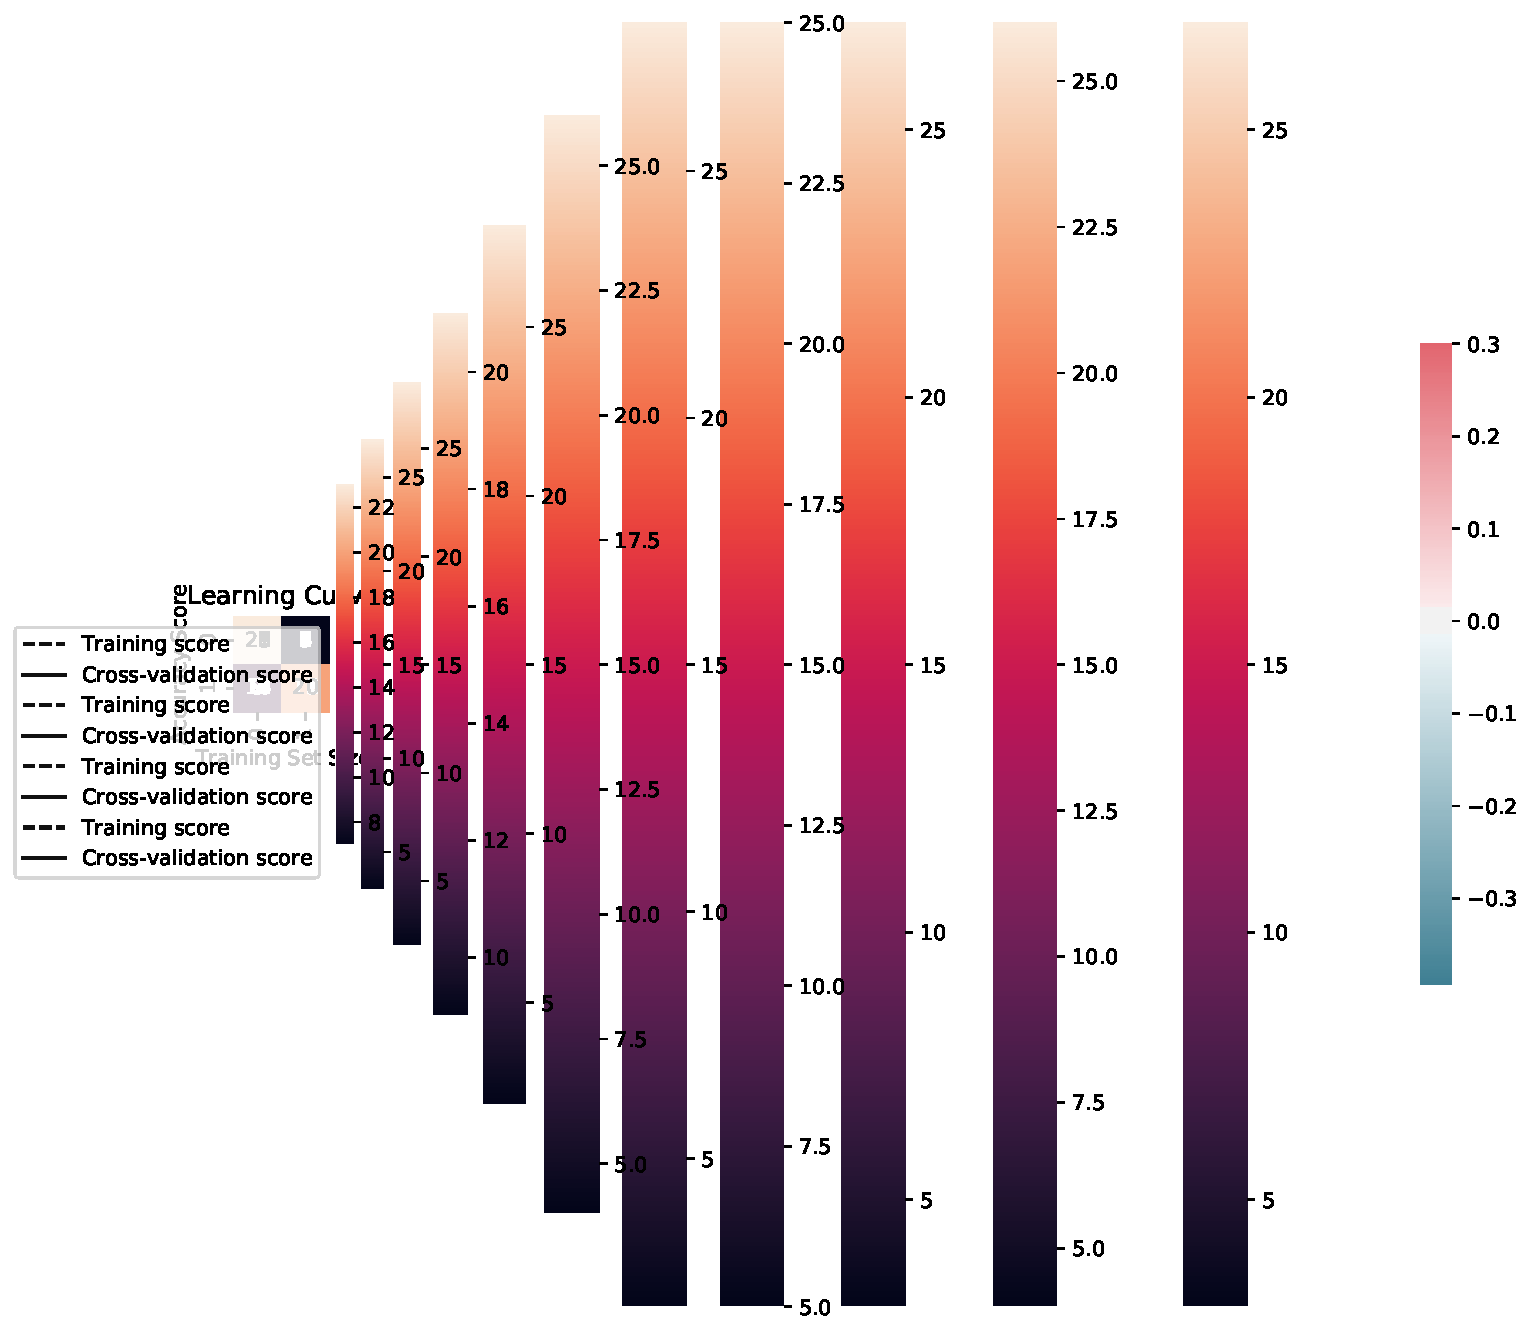
\includegraphics[width=0.9\linewidth]{images/DecisionTreeClassifier_lc.pdf}}
    \caption{Decision Tree Learning Curve}
    \label{dt_lc}
\end{figure}

\noindent
Max depth = 3\\
Train accuracy: 85.54%
\\Test accuracy: 78.69%
\\Number of mislabeled points out of a total 61 points : 13
\\The accuracy score achieved is: 78.69 %
\begin{table}[H]
\caption{Classification report on full data set:}
\begin{center}
\begin{tabular}{lrrrr}
\toprule
{} &  precision &  recall &  f1-score &  support \\
\midrule
0            &       0.79 &    0.86 &      0.82 &    35.00 \\
1            &       0.78 &    0.69 &      0.73 &    26.00 \\
accuracy     &       0.79 &    0.79 &      0.79 &     0.79 \\
macro avg    &       0.79 &    0.77 &      0.78 &    61.00 \\
weighted avg &       0.79 &    0.79 &      0.78 &    61.00 \\
\bottomrule
\end{tabular}

\label{decision_tree_class}
\end{center}
\end{table}
\noindent
False Negative Rate: 30.77
\\False Positive Rate: 14.29


\begin{figure}[H]
    \centerline{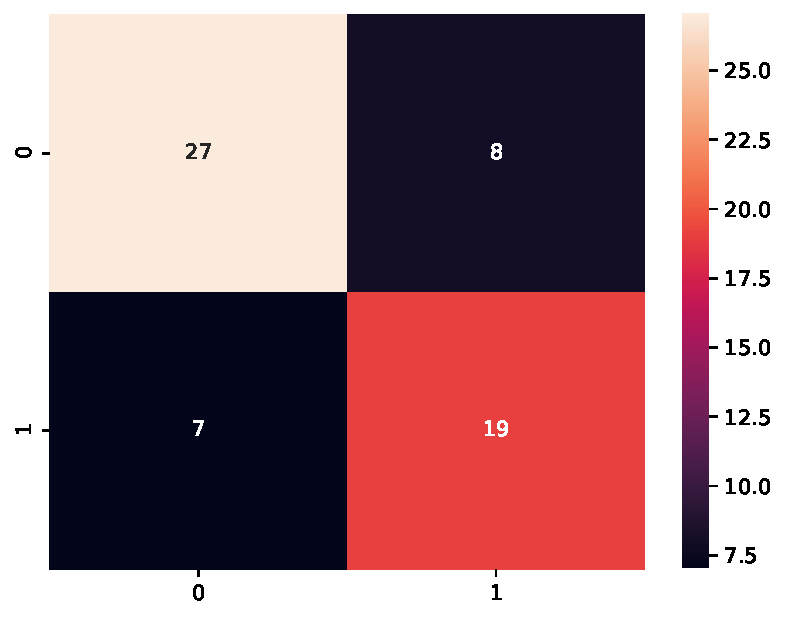
\includegraphics[width=0.8\linewidth]{images/decision_tree_cm.pdf}}
    \caption{Decision Tree Confusion Matrix}
    \label{dt_cm}
\end{figure}

\subsection{Random Forest}

A random forest is a meta estimator that fits a number of decision tree classifiers on various sub-samples of the dataset and uses averaging to improve the predictive accuracy and control over-fitting. The optimal value between processing time and accuracy is 100 trees and the depth of each tree was tested for 10 values, being the depth of 1 the one that provided the best results.

\begin{figure}[H]
    \centerline{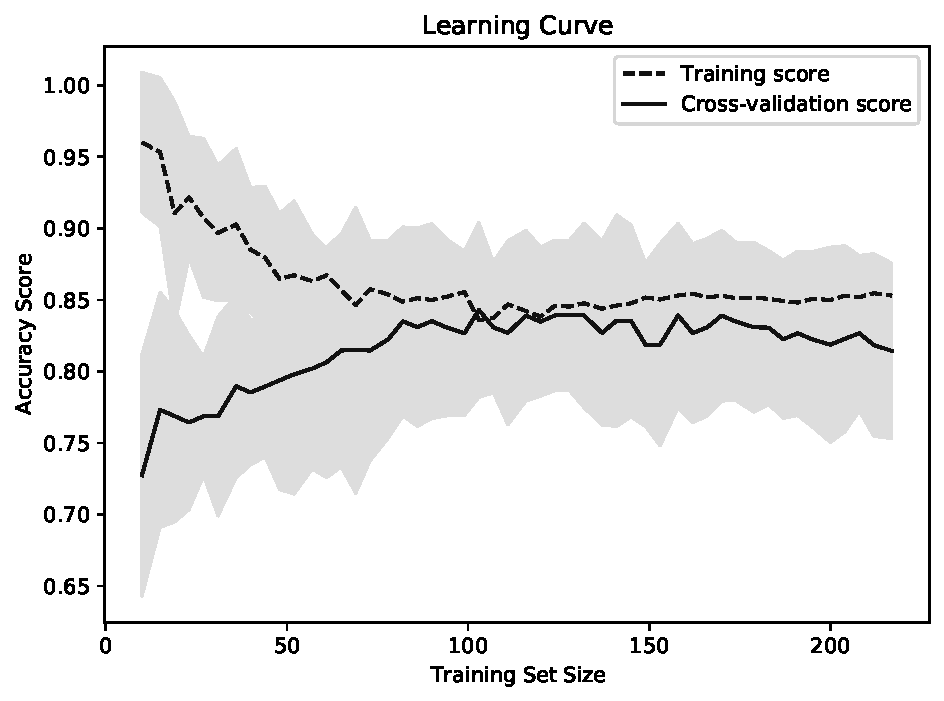
\includegraphics[width=0.9\linewidth]{images/RandomForestClassifier_lc.pdf}}
    \caption{Random Forest Learning Curve}
    \label{rf_lc}
\end{figure}

\noindent
Max depth = 1\\
Train accuracy: 84.30%
\\Test accuracy: 81.97%
\\Number of mislabeled points out of a total 61 points : 11
\\The accuracy score achieved is: 81.97 %
\begin{table}[H]
\caption{Classification report on full data set:}
\begin{center}
\begin{tabular}{lrrrr}
\toprule
{} &  precision &  recall &  f1-score &  support \\
\midrule
0            &       0.79 &    0.94 &      0.86 &    35.00 \\
1            &       0.89 &    0.65 &      0.76 &    26.00 \\
accuracy     &       0.82 &    0.82 &      0.82 &     0.82 \\
macro avg    &       0.84 &    0.80 &      0.81 &    61.00 \\
weighted avg &       0.83 &    0.82 &      0.81 &    61.00 \\
\bottomrule
\end{tabular}

\label{random_forest_class}
\end{center}
\end{table}
\noindent
False Negative Rate: 34.62
\\False Positive Rate: 5.71


\begin{figure}[H]
    \centerline{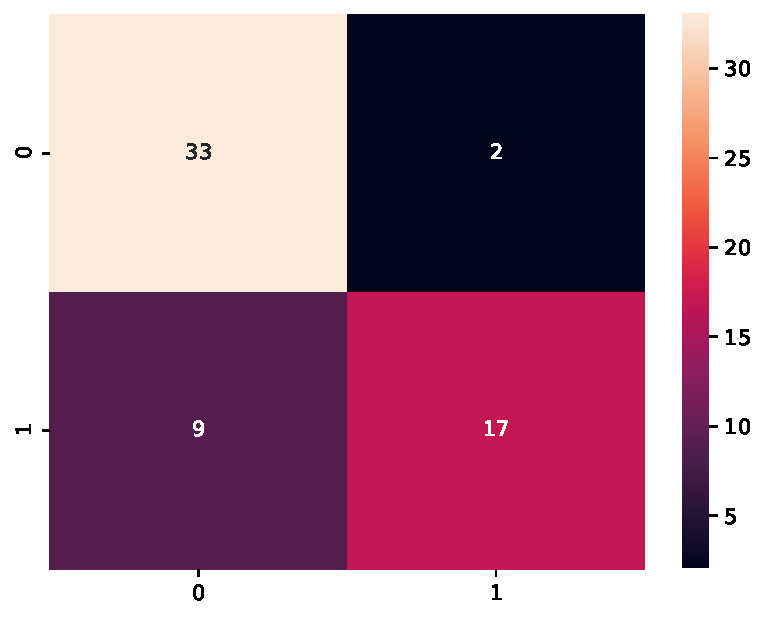
\includegraphics[width=0.8\linewidth]{images/random_forest_cm.pdf}}
    \caption{Random Forest Confusion Matrix}
    \label{rf_cm}
\end{figure}

\section{Results}

Here we can see the comparison between the models for both the original dataset and some different ones from other hospitals.

\begin{table}[H]
    \caption{Results for the test section of the original data}
    \begin{center}
        \begin{tabular}{lr}
\toprule
{} &  accuracy \\
\midrule
Random Forests      &     81.97 \\
Logistic Regression &     80.33 \\
Naive Bayes         &     78.69 \\
Decision Trees      &     78.69 \\
KNN                 &     70.49 \\
\bottomrule
\end{tabular}


        \label{ori_res}
    \end{center}
\end{table}

In Table \ref{ori_res} are the results taken from the evaluation of 20\% of the data, which was left out from the original dataset for these tests. We can see that Decision Trees and random Forest gave us the best results while Logistic Regression and K Nearest Neighbors fell short.

\begin{table}[H]
    \caption{Results for the V.A. Medical Center's data}
    \begin{center}
        \begin{tabular}{lr}
\toprule
{} &  accuracy \\
\midrule
Naive Bayes         &      72.5 \\
Decision Trees      &      68.0 \\
Random Forests      &      64.5 \\
Logistic Regression &      61.5 \\
KNN                 &      47.0 \\
\bottomrule
\end{tabular}


        \label{va_res}
    \end{center}
\end{table}

In another hospital from the USA\cite{va}, whose results are shown in Table \ref{va_res}, we have some general decrease on accuracy, but the relative efficiency of the models remains the same except for the K Nearest Neighbors with a 20\% drop on accuracy.

\begin{table}[H]
    \caption{Results for the Swiss data}
    \begin{center}
        \begin{tabular}{lr}
\toprule
{} &  accuracy \\
\midrule
Decision Trees      &     85.37 \\
Naive Bayes         &     73.98 \\
Random Forests      &     60.98 \\
Logistic Regression &     53.66 \\
KNN                 &     12.20 \\
\bottomrule
\end{tabular}


        \label{sw_res}
    \end{center}
\end{table}

Taking the data gathered by 2 hospitals in Switzerland\cite{swz1,swz2}, we see in Table \ref{sw_res} that Logistic Regression predicts most of the cases wrong while the rest of the models perform as expected.

\begin{table}[H]
    \caption{Results for the Hungarian data}
    \begin{center}
        \begin{tabular}{lr}
\toprule
{} &  accuracy \\
\midrule
Random Forests      &     82.99 \\
Logistic Regression &     81.97 \\
Naive Bayes         &     81.97 \\
Decision Trees      &     78.57 \\
KNN                 &     63.95 \\
\bottomrule
\end{tabular}


        \label{hun_res}
    \end{center}
\end{table}

The results taken from the data gathered by the Hungarian hospital\cite{hun} and displayed in Table \ref{hun_res} show a massive drop in accuracy from the Decision Tree and Logistic Regression and only Naive Bayes and Random Forest provided useful predictions.

\section{Conclusion}

Given the results, we can conclude that the model that gave the overall best results was the Random Tree, but this is also the most computational demanding and time consuming method. The Bernoulli Naive Bayes gave us good results to fit this specific dataset and it is simpler and lighter to implement so it seems to be the best choice.
\\The dataset used for training was relatively small so most of the models didn't have enough data to converge and provide us with a reliable prediction and the datasets tested the models with were missing many of its attributes, so some of the results may be misleading.

\begin{thebibliography}{00}
    \bibitem{hun} Hungarian Institute of Cardiology. Budapest: Andras Janosi, M.D.
    \bibitem{swz1} University Hospital, Zurich, Switzerland: William Steinbrunn, M.D.
    \bibitem{swz2} University Hospital, Basel, Switzerland: Matthias Pfisterer, M.D.
    \bibitem{va} V.A. Medical Center, Long Beach and Cleveland Clinic Foundation:Robert Detrano, M.D., Ph.D.
    \bibitem{mlr} Dua, D. and Graff, C. (2019). UCI Machine Learning Repository [http://archive.ics.uci.edu/ml]. Irvine, CA: University of California, School of Information and Computer Science.
\end{thebibliography}

\end{document}
